
%=================================================================
%                           Start Document
%=================================================================
\sectiontitle{2}{Introduction}
\lhead{Introduction} % section header

\setstretch{1.4}


\subsection{Motivation}
\lhead{Introduction - Motivation}

Navigating biomedical instruments inside the brain remains challenging and high-risk due to the complexity and sensitivity of neural tissue. A range of neurological conditions, including epilepsy, parkinson's and brain tumors such as glioblastoma often necessitate interventions that require very high precision for localized drug delivery, thermal ablation, targeted stimulation or intracranial monitoring. Epilepsy alone affects around 50 million people globally \cite{noauthor_epilepsy_nodate}, and for nearly a third of them, medication alone is not enough to control seizures \cite{sultana_incidence_2021}. Glioblastoma, one of the most aggressive forms of brain cancer is diagnosed in approximately 150 000 people each year \cite{walsh_chapter_2016} may of which are deemed inoperable with traditional surgical tools. Finally many of the 10 million worldwide parkinsons patients \cite{noauthor_statistics_nodate} rely on precise deep brain stimulation to alleviate debilitating symptoms. There is thus a clear real-world benefit to be made by improving the precision, safety, and accessibility of technologies that enable minimally invasive, targeted brain interventions.

Robotic-assisted surgery has transformed many fields, but its application in neurosurgery remains limited by current technology \cite{doulgeris_robotics_2015}.The traditional rigid instruments are restricted in their ability to navigate delicate and structurally complex soft tissues such as the brain \cite{noseda_flat_2024}. Steerable, flexible devices offer a potential solution, improving access and safety while enabling new procedures \cite{da_veiga_challenges_2020}. Small-scale robotic devices, particularly those designed for transcranial access (see figure \ref{fig:transcranialvsendocascular}) offer a new way to reach deep seated brain regions with minimal disruption. Unlike endovascular methods, transcranial routes allow more flexibility in choosing paths.
\begin{figure} [H]
    \centering
    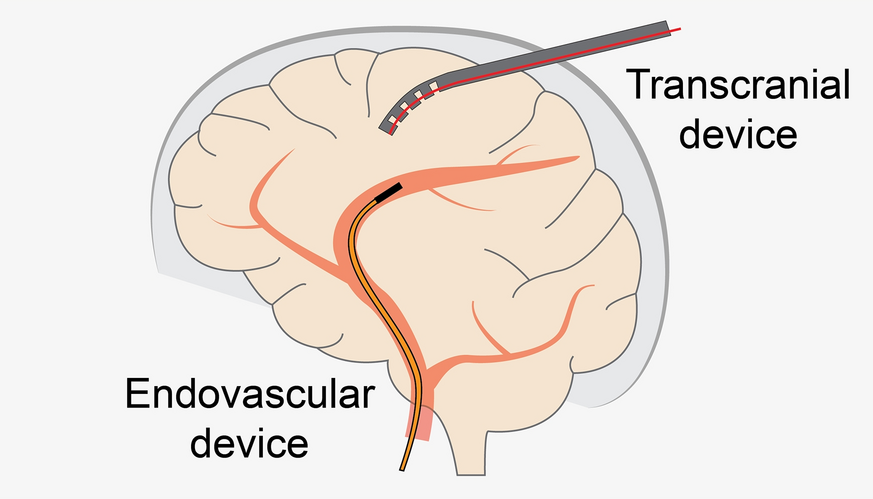
\includegraphics[width=0.8\linewidth]{images/brain surgery/43577_2023_644_Figa_HTML.png}
    \caption{Visualization of transcranial vs endovascular devices}
    \label{fig:transcranialvsendocascular}
\end{figure}

Additionally, advancements in microfabrication have enabled the production of microscopic probes capable of monitoring biological activity and delivering stimulation or therapy \cite{chen_neural_2017} \cite{frank_next-generation_2019}.  However, no existing device has successfully combined these emerging technologies with the unique potential of steerable, flexible instruments for neurosurgery. A device that integrates both would enable real-time sensing and targeted treatment while navigating delicate brain structures.

To address this unmet need the MICROBS lab has developed a novel ribbon-shaped, tendon-driven continuum microrobot for minimally invasive neurosurgical interventions. This design allows for agile 3D navigation by achieving configuration unattainable by traditional rod-like instruments \cite{noseda_flat_2024}. Enabling precise navigation through soft tissue, capable of safely avoiding critical structures and reaching multiple targets in a single insertion.  Furthermore, the flat, ribbon-like geometry is well suited for integrating the emerging microfabricated technologies, such as embedded sensors or therapeutic elements, along its surface. However, this unique geometry introduces new challenges in modeling and control, requiring specialized solutions. 

Due to the flexibility of these devices and the complex, deformable nature of brain tissue, reliable closed-loop control is essential for accurate navigation. Flexible continuum robots continuously interact with their surroundings, making their motion highly sensitive to tissue deformation, friction, and anatomical variability. As a result, their behavior is expected to be non-intuitive for a surgeon to control directly through manual operation, making automated path-following under surgical supervision, the most practical approach.

Beyond the technical necessity of closed-loop navigation, such automated systems could also help address the global shortage of neurosurgical expertise. More than 80\% of the estimated 14 million neurosurgical cases that develop each year arise in low- and middle-income countries, where the ratio of neurosurgeons to neurosurgical disease is critically low \cite{dewan_global_2019}. Automation technologies that reduce reliance on specialist manual skills have the potential to improve access to care for the approximately 5 million people each year who suffer from treatable neurosurgical conditions but never receive surgical intervention \cite{dewan_global_2019}.

Recognizing this need, the aim of this thesis is to develop closed-loop navigation for the novel ribbon-robotic device enabling future effective use of this technology for brain surgery. 


\lhead{Introduction - Project Interpretation}
\subsection{Project Interpretation}
In addition to the main goal of closed-loop navigation several preliminary tasks, outlined as  as steps 1-4 in the project description, needed to be completed. This made the scope of the project quite broad, but the primary goal was to produce reliable, well-documented work rooted in established theory. Early on, it was therefore agreed that if necessary, certain tasks could be omitted to allow for a more thorough solution to the remaining ones. This was an important tradeoff to ensure that the project could serve as a solid foundation for further development and function as a robust proof of concept that could be used for demonstration to both clinicians and engineers.

To the best of the author's knowledge, this is the first system of its kind and it thereby poses new and significant control challenges. As such, a substantial portion of the project needed to be spent on developing the mathematical foundations of the system. Given the project's limited time frame and the number of prerequisite tasks, it was decided that focus would be on implementing a robust 2D control strategy rather than rushing to implement a full 3D solution. Special attention was also given to implementing the system in a robust and modular way in the codebase. The overall goal being to deliver a reusable, scalable system that avoids the need for major rework in future development, rather than pursuing a more complex solution at the cost of quality or maintainability. 

\subsection{Project Context}
\lhead{Introduction - Project Context}
This thesis builds upon an ongoing research project at the MICROBS lab at EPFL towards developing a novel ribbon-shaped, tendon-driven continuum microrobot for minimally invasive neurosurgical interventions. The request for a closed-loop control mechanism for the device came from Lorenzo Noseda, who designed both the ribbon device and its robotic platform as part of his PhD work at the lab. 

In addition to using the existing hardware, this work also utilizes software developed by previous students. This includes a path planning algorithm specifically tailored to the device, as well as a Python-based 3D tip-tracking vision algorithm, which provides visual feedback for the system. There was also an existing control code base for the first iteration of the hardware, however this did not include a navigation system and did not incorporate the path planning and tip tracking. The code base therefore had to refactored and the path planning and tip tracking integrated into the system.


\subsection{Contributions}
\lhead{Introduction - Contributions}
The contributions of this thesis lie in the development and implementation of a closed-loop navigation system for the novel ribbon-shaped robotic device. To achieve this, a modular and C++ control software with a scalable architecture was developed. A python-based real-time 2D tip-tracking vision system was incorporated into the control software through a custom communication framework, providing the necessary feedback for closed-loop control. A previously developed path planning algorithm was also incorporated into the system, allowing the robot to follow pre-defined trajectories.

The inner tendon tension control system was significantly improved, achieving robust and stable closed-loop performance. Thorough experimental validation demonstrated very minimal errors (<1mN) while moving with a constant tension setpoint and reliable tracking of ramped setpoints.

Finally, building on these foundations, a 2D path-following system was developed and implemented, combining kinematic modeling, closed-loop pitch control, and a curved Integral Line-Of-Sight (ILOS) guidance method, a novel application of this type of guidance system. Experimental validation in a brain phantom demonstrated accurate and stable path-following performance with consistent sub-0.1mm precision, even when following curved trajectories. This work provides a significant proof of concept for the kinematic modeling proposed in the thesis, the use of ILOS for such a system and of the navigation capabilities of the device for possible future use in neurosurgical applications.


\subsection{Outline}
\lhead{Introduction - Outline}
This work is structured into first the introduction which outlines the motivation behind the research, the project scope and objectives. Thereafter there is a Hardware section that describes the physical hardware that is used for the subsequent development.

The main body of the thesis is divided into five core topics corresponding to tasks 1-5 in the project description. These sections generally include methods, implementation and discussion with some also featuring design and further work subsections. The main section on 2D navigation is the last of these, and readers only interested in the background and analysis of the final navigation of the system are recommended to read the hardware section and then jump to the 2D path-following section.

The first topic is software refactoring, detailing the methodology for the restructuring and development of the software framework. The second section describes how the tip tracking vision system was refactored and integrated with the control system. The third section focuses on how the existing path planning system was integrated with the 2D path following system. The fourth topic explains how the closed-loop tension control for the individual tendons was implemented and discusses its performance. The fifth and final section addresses the final 2D path following system, this is also where the major background section and literature review is done for this thesis. The section also describes the design, kinematic modeling, implementation, and evaluation of the closed-loop system, along with an interpretation of the results, and discussion on possible further work. Conclusion wise, there is brief section which summarizes the project and reflects on its results.


%==============================================================
%                           End Document
%==============================================================
